\documentclass[11pt,aspectratio=169]{beamer}
%\documentclass[11pt,aspectratio=169,handout]{beamer}

\input{../Macros/main}
\subtitle{\vspace{2.1em}Lecture 5: Games in Extensive Form}

\begin{document}

 \begin{frame}[plain]
  \titlepage
 \end{frame}
 
 \section{Perfect-info Extensive-form Games}
 
  \begin{frame}{Extensive-form Games}
   \begin{itemize}[<+->]
   \setlength{\itemsep}{1.5em}
    \item So far, we have studied \alert{strategic-form} games
    \begin{itemize}[<.->]
     \item Agents take actions once and simultaneously
    \end{itemize}
    \item Next, we study \alert{extensive-form} games (a.k.a. \alert{sequential} or \alert{multi-stage} games)
    \begin{itemize}[<.->]
     \item Extensive-form games can be conveniently represented by \alert{game trees}
    \end{itemize}
   \end{itemize}
  \end{frame}
  
  
  \begin{frame}{(Finite) Perfect-info Extensive-form Game: Definition}
   \begin{itemize}[<+->]
   \setlength{\itemsep}{1.2em}
    \item The game consists of a set of agents, $N=\{1,2,\dots,n\}$
    \item $A$ is set of actions
    \item $H$ is set of \alert{choice nodes} (internal nodes of game tree)
    \item $Z$ is set of \alert{terminal} nodes (leaves of game tree)
   \end{itemize}
  \end{frame}  
  
  
  \begin{frame}{(Finite) Perfect-info Extensive-form Game: Definition (cont.)}
   \begin{itemize}[<+->]
   \setlength{\itemsep}{1em}
    \item $\alpha : H \rightarrow N$ is \alert{agent function}
    \begin{itemize}[<.->]
     \item Maps each choice node to an agent who chooses an action at that node
    \end{itemize}
    \item $\beta : H \rightarrow 2^{A}$ is \alert{action function}
    \begin{itemize}[<.->]
     \item Maps each choice node to set of actions available at that node
    \end{itemize}
    \item $\rho: H \times A \rightarrow H \cup Z$ is \alert{successor function}
    \begin{itemize}[<.->]
     \item Maps each choice node and action pair to new choice node or terminal node
     \item If $\rho(h_1, a_1) = \rho(h_2, a_2)$ then $h_1 = h_2$ and $a_1 = a_2$
    \end{itemize}
    \item $u = (u_1, \dots, u_n)$, where $u_i: Z \rightarrow \mathbb{R}$ is agent $i$'s \alert{utility function}
    \begin{itemize}[<.->]
     \item Maps each terminal node to a real value
    \end{itemize}
   \end{itemize}
  \end{frame} 
  
  
  \begin{frame}{Example: Sharing Game}
   \begin{columns}
    \begin{column}{0.5\textwidth}
     \begin{itemizes}
      \item Brother and sister share two gifts
      \item Brother suggests a split first
      \item Sister then chooses to accept or reject
      \item If she accepts, they get suggested gifts
      \item Otherwise, neither gets any gift
     \end{itemizes}
    \end{column}
    \begin{column}{0.5\textwidth}
     \begin{center} \tiny
      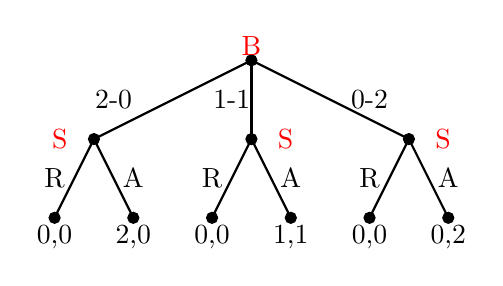
\begin{tikzpicture}[x=0.5cm,y=0.5cm]
       \filldraw[black] (5,4) circle (2pt) node[anchor=north, yshift=12pt, color=red]{B};
       \filldraw[black] (1,2) circle (2pt) node[anchor=east, xshift=-6pt, color=red]{S};
       \filldraw[black] (5,2) circle (2pt) node[anchor=west, xshift=6pt, color=red]{S};
       \filldraw[black] (9,2) circle (2pt) node[anchor=west, xshift=6pt, color=red]{S};      
       \filldraw[black] (0,0) circle (2pt) node[] at (0,-0.5) {0,0}; 
       \filldraw[black] (2,0) circle (2pt) node[] at (2,-0.5) {2,0};
       \filldraw[black] (4,0) circle (2pt) node[] at (4,-0.5) {0,0};
       \filldraw[black] (6,0) circle (2pt) node[] at (6,-0.5) {1,1};
       \filldraw[black] (8,0) circle (2pt) node[] at (8,-0.5) {0,0};
       \filldraw[black] (10,0) circle (2pt) node[] at (10,-0.5) {0,2};      
       \draw[black, thick] (5,4) -- (1, 2) node[] at (1.5, 3) {2-0};
       \draw[black, thick] (5,4) -- (5, 2) node[] at (4.5, 3) {1-1};
       \draw[black, thick] (5,4) -- (9, 2) node[] at (8, 3) {0-2};
       \draw[black, thick] (1,2) -- (0, 0) node[] at (0, 1) {R}; 
       \draw[black, thick] (1,2) -- (2, 0) node[] at (2, 1) {A};
       \draw[black, thick] (5,2) -- (4, 0) node[] at (4, 1) {R};
       \draw[black, thick] (5,2) -- (6, 0) node[] at (6, 1) {A};
       \draw[black, thick] (9,2) -- (8, 0) node[] at (8, 1) {R};
       \draw[black, thick] (9,2) -- (10, 0) node[] at (10, 1) {A};
      \end{tikzpicture}
     \end{center}
    \end{column}
   \end{columns}
  \end{frame}
  
  
 \section{Pure Strategies in Perfect-info Games}
 
  \begin{frame}{History in Extensive-form Games}
   \begin{itemizes}\small
    \item If height of game tree (i.e, number of stages) is finite, then game is \alert{finite-horizon} game
    \item Otherwise, the game is called \alert{infinite-horizon} game
    \item For perfect-information games, each node maps to unique history (and vice versa)
    \item Since choice nodes form a tree, we can unambiguously identify a node with its history
    \begin{itemize}
     \item I.e., sequence of choices leading from the root node to it
    \end{itemize}
   \end{itemizes}
  \end{frame} 
 
  \begin{frame}{Pure Strategies}
   \begin{itemizes}
    \item Agent $i$'s pure strategy defines contingency plan for \alert{\underline{all}} choice nodes mapped to $i$
    $$ a_i \in A_i = \prod_{h \in H, \alpha(h) = i}\beta(h) $$
    \item Strategy must specify a decision at each choice node
    \begin{itemize}
     \item Regardless of whether it is possible to reach that node
    \end{itemize}
   \end{itemizes}
  \end{frame}


  \begin{frame}{Pure Strategies: Example}
   \begin{center} \tiny
    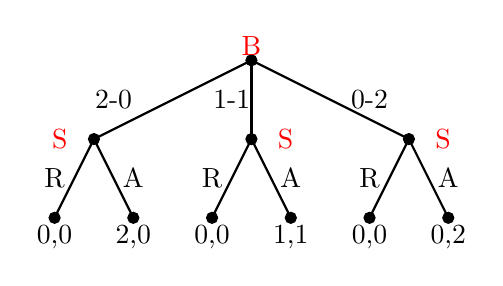
\begin{tikzpicture}[x=0.5cm,y=0.5cm]
     \filldraw[black] (5,4) circle (2pt) node[anchor=north, yshift=12pt, color=red]{B};
     \filldraw[black] (1,2) circle (2pt) node[anchor=east, xshift=-6pt, color=red]{S};
     \filldraw[black] (5,2) circle (2pt) node[anchor=west, xshift=6pt, color=red]{S};
     \filldraw[black] (9,2) circle (2pt) node[anchor=west, xshift=6pt, color=red]{S};      
     \filldraw[black] (0,0) circle (2pt) node[] at (0,-0.5) {0,0}; 
     \filldraw[black] (2,0) circle (2pt) node[] at (2,-0.5) {2,0};
     \filldraw[black] (4,0) circle (2pt) node[] at (4,-0.5) {0,0};
     \filldraw[black] (6,0) circle (2pt) node[] at (6,-0.5) {1,1};
     \filldraw[black] (8,0) circle (2pt) node[] at (8,-0.5) {0,0};
     \filldraw[black] (10,0) circle (2pt) node[] at (10,-0.5) {0,2};      
     \draw[black, thick] (5,4) -- (1, 2) node[] at (1.5, 3) {2-0};
     \draw[black, thick] (5,4) -- (5, 2) node[] at (4.5, 3) {1-1};
     \draw[black, thick] (5,4) -- (9, 2) node[] at (8, 3) {0-2};
     \draw[black, thick] (1,2) -- (0, 0) node[] at (0, 1) {R}; 
     \draw[black, thick] (1,2) -- (2, 0) node[] at (2, 1) {A};
     \draw[black, thick] (5,2) -- (4, 0) node[] at (4, 1) {R};
     \draw[black, thick] (5,2) -- (6, 0) node[] at (6, 1) {A};
     \draw[black, thick] (9,2) -- (8, 0) node[] at (8, 1) {R};
     \draw[black, thick] (9,2) -- (10, 0) node[] at (10, 1) {A};
    \end{tikzpicture}
   \end{center}
   \vspace{1cm}
   \begin{itemize}\footnotesize
    \item $A_B=\{$``2-0'', ``1-1'', ``0-2''$\}$
    \item $A_S=\{$(R, R, R), (R, R, A), (R, A, R), (A, R, R), (R, A, A), (A, R, A), (A, A, R), (A, A, A)$\}$
   \end{itemize}
  \end{frame}
  
  
  \begin{frame}{Pure Strategies: (Another) Example}
   \begin{columns}
    \begin{column}{0.6\textwidth}
     \begin{itemize}[<+->]
     \setlength{\itemsep}{1.5em}
      \item What are pure strategies for A2?
      \begin{itemize}
       \item $A_{A2} = \{$(L, L), (L, R), (R, L), (R, R)$\}$
      \end{itemize}
      \item What about A1?
      \begin{itemize}
       \item $A_{A1} = \{$(L, L), (L, R), (R, L), (R, R)$\}$
      \end{itemize}
     \end{itemize}
    \end{column}
    \begin{column}{0.4\textwidth}\tiny
     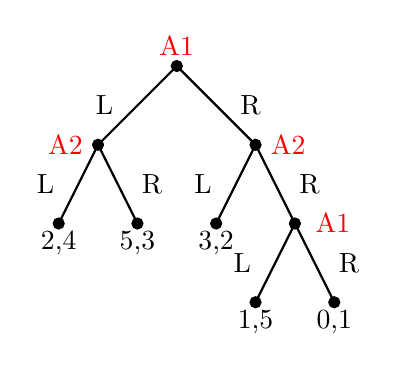
\begin{tikzpicture}[x=0.5cm,y=0.5cm,step=0.5cm]
      \filldraw[black] (3,6) circle (2pt) node[red] at (3, 6.5) {A1};   
      \filldraw[black] (1,4) circle (2pt) node[red, left=2pt] at (1, 4) {A2};
      \filldraw[black] (5,4) circle (2pt) node[red, right=2pt] at (5, 4) {A2};   
      \filldraw[black] (0,2) circle (2pt) node[] at (0,1.5) {2,4};
      \filldraw[black] (2,2) circle (2pt) node[] at (2,1.5) {5,3};
      \filldraw[black] (4,2) circle (2pt) node[] at (4,1.5) {3,2};
      \filldraw[black] (6,2) circle (2pt) node[red, right=4pt] at (6,2) {A1};   
      \filldraw[black] (5,0) circle (2pt) node[] at (5,-0.5) {1,5};
      \filldraw[black] (7,0) circle (2pt) node[] at (7,-0.5) {0,1};
      \draw[black, thick] (3,6) -- (1, 4) node[left=5pt] at (2, 5) {L};
      \draw[black, thick] (3,6) -- (5, 4) node[right=5pt] at (4, 5) {R};   
      \draw[black, thick] (1,4) -- (0, 2) node[left=5pt] at (0.5, 3) {L};
      \draw[black, thick] (1,4) -- (2, 2) node[right=5pt] at (1.5, 3) {R};     
      \draw[black, thick] (5,4) -- (6, 2) node[right=5pt] at (5.5, 3) {R};
      \draw[black, thick] (5,4) -- (4, 2) node[left=5pt] at (4.5, 3) {L};   
      \draw[black, thick] (6,2) -- (5, 0) node[left=5pt] at (5.5, 1) {L};
      \draw[black, thick] (6,2) -- (7, 0) node[right=5pt] at (6.5, 1) {R};    
     \end{tikzpicture}
    \end{column}
   \end{columns}
  \end{frame}


  \begin{frame}{Normal-form Representation of Extensive-form Games}
   \begin{itemize}
    \item For every perfect-info game, there is corresponding normal-form game
   \end{itemize}
   \vspace{1cm}
   \begin{columns}
    \begin{column}{0.6\textwidth}
     \begin{center}\scriptsize
      \begin{game}{4}{4}[A1][A2]
      			\>	(L, L)	\>	(L, R)	\>	(R, L)	\>	(R, R)	\\
       (L, L)	\>	$2, 4$	\>	$2, 4$	\>	$5, 3$	\>	$5, 3$	\\
       (L, R)	\>	$2, 4$	\>	$2, 4$	\>	$5, 3$	\>	$5, 3$	\\
       (R, L)	\>	$3, 2$	\>	$1, 5$	\>	$3, 2$	\>	$1, 5$	\\
       (R, R)	\>	$3, 2$	\>	$0, 1$	\>	$3, 2$	\>	$0, 1$	
      \end{game}
     \end{center}
    \end{column}
    \begin{column}{0.4\textwidth}\tiny
     \vspace{-1cm}
     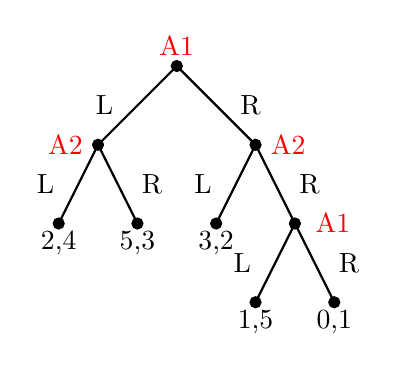
\begin{tikzpicture}[x=0.5cm,y=0.5cm,step=0.5cm]
      \filldraw[black] (3,6) circle (2pt) node[red] at (3, 6.5) {A1};   
      \filldraw[black] (1,4) circle (2pt) node[red, left=2pt] at (1, 4) {A2};
      \filldraw[black] (5,4) circle (2pt) node[red, right=2pt] at (5, 4) {A2};   
      \filldraw[black] (0,2) circle (2pt) node[] at (0,1.5) {2,4};
      \filldraw[black] (2,2) circle (2pt) node[] at (2,1.5) {5,3};
      \filldraw[black] (4,2) circle (2pt) node[] at (4,1.5) {3,2};
      \filldraw[black] (6,2) circle (2pt) node[red, right=4pt] at (6,2) {A1};   
      \filldraw[black] (5,0) circle (2pt) node[] at (5,-0.5) {1,5};
      \filldraw[black] (7,0) circle (2pt) node[] at (7,-0.5) {0,1};
      \draw[black, thick] (3,6) -- (1, 4) node[left=5pt] at (2, 5) {L};
      \draw[black, thick] (3,6) -- (5, 4) node[right=5pt] at (4, 5) {R};   
      \draw[black, thick] (1,4) -- (0, 2) node[left=5pt] at (0.5, 3) {L};
      \draw[black, thick] (1,4) -- (2, 2) node[right=5pt] at (1.5, 3) {R};     
      \draw[black, thick] (5,4) -- (6, 2) node[right=5pt] at (5.5, 3) {R};
      \draw[black, thick] (5,4) -- (4, 2) node[left=5pt] at (4.5, 3) {L};   
      \draw[black, thick] (6,2) -- (5, 0) node[left=5pt] at (5.5, 1) {L};
      \draw[black, thick] (6,2) -- (7, 0) node[right=5pt] at (6.5, 1) {R};    
     \end{tikzpicture}
    \end{column}
   \end{columns}
  \end{frame}


  \begin{frame}{Transformation from Extensive form to Normal From}
   \begin{itemizes}
    \item It can \alert{always} be performed for perfect-information games
    \item It can cause redundancy
    \begin{itemize}
     \item E.g., $(2, 4)$ occurs once in extensive form but 4 times in normal form
    \end{itemize}
    \item It can result in \alert{exponential blowup} of game representation
    \item Reverse transformation does not always exist
    \begin{itemize}
     \item E.g., there is \alert{no} extensive-form representation for Prisoner's Dilemma
     \item Perfect-information extensive-form games cannot model \alert{simultaneity}
    \end{itemize}
   \end{itemizes}
  \end{frame}

 
  \begin{frame}{Nash Equilibrium of Perfect-info Games in Extensive Form}
   \begin{itemize}
   \setlength{\itemsep}{1.5em}
    \item \alert{[Theorem]} Every (finite) perfect-info extensive-form game has \alert{pure-strategy} NE
    \item Agents see everything before each action $\Rightarrow$ randomness is not required
    \item This is not the case for every finite game in normal form
   \end{itemize}
  \end{frame}
  
  
  \begin{frame}{Nash Equilibrium: An Empty Threat?}
   \begin{columns}
    \begin{column}{0.6\textwidth}
     \begin{center}\scriptsize
      \begin{game}{4}{4}[A1][A2]
      			\>	(L, L)	\>	(L, R)	\>	(R, L)	\>	(R, R)	\\
       (L, L)	\>	$2, 4$	\>	\nebox[]{$2, 4$}	\>	$5, 3$	\>	$5, 3$	\\
       (L, R)	\>	$2, 4$	\>	\nebox[]{$2, 4$}	\>	$5, 3$	\>	$5, 3$	\\
       (R, L)	\>	$3, 2$	\>	$1, 5$	\>	$3, 2$	\>	$1, 5$	\\
       (R, R)	\>	\only<1>{\nebox[]{$3, 2$}}\only<2->{\nebox[red,]{$3, 2$}}	\>	$0, 1$	\>	$3, 2$	\>	$0, 1$	
      \end{game}
     \end{center}
    \end{column}
    \begin{column}{0.4\textwidth}\tiny
     \vspace{-1cm}
     \begin{tikzpicture}[x=0.5cm,y=0.5cm,step=0.5cm]
      \only<1>{\draw[black, thick] (3,6) -- (1, 4) node[left=5pt] at (2, 5) {L};
      \draw[black, thick] (3,6) -- (5, 4) node[right=5pt] at (4, 5) {R};   
      \draw[black, thick] (1,4) -- (0, 2) node[left=5pt] at (0.5, 3) {L};
      \draw[black, thick] (1,4) -- (2, 2) node[right=5pt] at (1.5, 3) {R};     
      \draw[black, thick] (5,4) -- (6, 2) node[right=5pt] at (5.5, 3) {R};
      \draw[black, thick] (5,4) -- (4, 2) node[left=5pt] at (4.5, 3) {L};   
      \draw[black, thick] (6,2) -- (5, 0) node[left=5pt] at (5.5, 1) {L};
      \draw[black, thick] (6,2) -- (7, 0) node[right=5pt] at (6.5, 1) {R};}
      \only<2->{\draw[black, thick] (3,6) -- (1, 4) node[left=5pt] at (2, 5) {L};
      \draw[red, thick, line width=2pt] (3,6) -- (5, 4) node[right=5pt] at (4, 5) {R};   
      \draw[red, thick, line width=2pt] (1,4) -- (0, 2) node[left=5pt] at (0.5, 3) {L};
      \draw[black, thick] (1,4) -- (2, 2) node[right=5pt] at (1.5, 3) {R};     
      \draw[black, thick] (5,4) -- (6, 2) node[right=5pt] at (5.5, 3) {R};
      \draw[red, thick, line width=2pt] (5,4) -- (4, 2) node[left=5pt] at (4.5, 3) {L};   
      \draw[black, thick] (6,2) -- (5, 0) node[left=5pt] at (5.5, 1) {L};
      \draw[red, thick, line width=2pt] (6,2) -- (7, 0) node[right=5pt] at (6.5, 1) {R};}
      \filldraw[black] (3,6) circle (2pt) node[] at (3, 6.5) {A1};   
      \filldraw[black] (1,4) circle (2pt) node[left=2pt] at (1, 4) {A2};
      \filldraw[black] (5,4) circle (2pt) node[right=2pt] at (5, 4) {A2};   
      \filldraw[black] (0,2) circle (2pt) node[] at (0,1.5) {2,4};
      \filldraw[black] (2,2) circle (2pt) node[] at (2,1.5) {5,3};
      \filldraw[black] (4,2) circle (2pt) node[] at (4,1.5) {3,2};
      \filldraw[black] (6,2) circle (2pt) node[right=4pt] at (6,2) {A1};   
      \filldraw[black] (5,0) circle (2pt) node[] at (5,-0.5) {1,5};
      \filldraw[black] (7,0) circle (2pt) node[] at (7,-0.5) {0,1};     
     \end{tikzpicture}
    \end{column}
   \end{columns}
   \vspace{1cm}
   \begin{itemize}
    \item<3-> Strategy of A1 is called a \alert{threat}
    \begin{itemize}
     \item Committing to choose R forces A2 to avoid that part of the tree
    \end{itemize}
    \item<4-> A2 may not consider A1's threat to be \alert{credible}
    \begin{itemize}
     \item Would A1 really follow through on this threat if final decision node is reached?
    \end{itemize}
   \end{itemize}
  \end{frame}


 \section{Subgame-perfect Equilibrium}
 
  \begin{frame}{Subgames: Definition}
   \begin{itemize}
   \setlength{\itemsep}{1.5em}
    \item Let $G$ be a perfect-information extensive-form game
    \item \alert{Subgame} of $G$ rooted at node $h$ is restriction of $G$ to descendants of $h$
    \item Set of subgames of $G$ consists of all of subgames of $G$ rooted at some node in G
   \end{itemize}
  \end{frame}


  \begin{frame}{Subgames: Example} 
   {\tiny
    \begin{tikzpicture}[x=0.5cm,y=0.5cm,step=0.5cm,remember picture, overlay,shift={(8,-10)}]
     \draw[black, thick] (3,6) -- (1, 4) node[left=5pt] at (2, 5) {L};
     \draw[black, thick] (3,6) -- (5, 4) node[right=5pt] at (4, 5) {R};   
     \draw[black, thick] (1,4) -- (0, 2) node[left=5pt] at (0.5, 3) {L};
     \draw[black, thick] (1,4) -- (2, 2) node[right=5pt] at (1.5, 3) {R};     
     \draw[black, thick] (5,4) -- (6, 2) node[right=5pt] at (5.5, 3) {R};
     \draw[black, thick] (5,4) -- (4, 2) node[left=5pt] at (4.5, 3) {L};   
     \draw[black, thick] (6,2) -- (5, 0) node[left=5pt] at (5.5, 1) {L};
     \draw[black, thick] (6,2) -- (7, 0) node[right=5pt] at (6.5, 1) {R};  
     \only<1,3->{\filldraw[black] (6,2) circle (2pt) node[right=4pt] at (6,2) {A1};}
     \only<2>{\filldraw[red] (6,2) circle (2pt) node[right=4pt] at (6,2) {A1};}
     \only<1-2,4->{\filldraw[black] (5,4) circle (2pt) node[right=2pt] at (5, 4) {A2};}
     \only<3>{\filldraw[red] (5,4) circle (2pt) node[right=2pt] at (5, 4) {A2};}
     \only<1-3,5>{\filldraw[black] (1,4) circle (2pt) node[left=2pt] at (1, 4) {A2};}
     \only<4>{\filldraw[red] (1,4) circle (2pt) node[left=2pt] at (1, 4) {A2};}
     \only<1-4>{\filldraw[black] (3,6) circle (2pt) node[] at (3, 6.5) {A1};}
     \only<5>{\filldraw[red] (3,6) circle (2pt) node[] at (3, 6.5) {A1};}
     \filldraw[black] (0,2) circle (2pt) node[] at (0,1.5) {2,4};
     \filldraw[black] (2,2) circle (2pt) node[] at (2,1.5) {5,3};
     \filldraw[black] (4,2) circle (2pt) node[] at (4,1.5) {3,2};
     \filldraw[black] (5,0) circle (2pt) node[] at (5,-0.5) {1,5};
     \filldraw[black] (7,0) circle (2pt) node[] at (7,-0.5) {0,1};   
     \visible<2->{\draw [-stealth, thick, white!60!black](7.2,1.7) -- (10,-1);}
     \visible<3->{\draw [-stealth, thick, white!60!black](6.2,3.8) -- (10,2.4);}
     \visible<4->{\draw [-stealth, thick, white!60!black](0.6,4.4) -- (-0.5,5.6);}
     \visible<5>{\draw [-stealth, thick, white!60!black](3.6,6.1) -- (10,7);}
    \end{tikzpicture}
   }
   \visible<2->{\tiny
    \begin{tikzpicture}[x=0.5cm,y=0.5cm,step=0.5cm, remember picture, overlay,shift={(19.8,-5)}]
     \draw[black, thick] (0,0) -- (0, -2);
     \draw[black, thick] (2,0) -- (2, -2);
     \draw[black, thick] (0,0) -- (2, 0);
     \draw[black, thick] (0,-1) -- (2, -1);
     \draw[black, thick] (0,-2) -- (2, -2);
   
   % ========== values ===2,4============
     \node[] at (1, -0.5) {1,5};
     \node[] at (1, -1.5) {0,1};
   
   % ========== cols ================
     \node[] at (1, 0.5) {(*, *)};
   
   % ========== rows ================
     \node[] at (-1, -0.5) {(*, L)};
     \node[] at (-1, -1.5) {(*, R)};
   
   % ========== titles ==============
     \node[] at (-2, -1) {A1};
     \node[] at (1, 1) {A2};
   
    \end{tikzpicture}
   }
   \visible<3->{\tiny
    \begin{tikzpicture}[x=0.5cm,y=0.5cm,step=0.5cm, remember picture, overlay,shift={(19.5,-1)}]
     \draw[black, thick] (0,0) -- (0, -2);
     \draw[black, thick] (2,0) -- (2, -2);
     \draw[black, thick] (4,0) -- (4, -2);
     \draw[black, thick] (0,0) -- (4, 0);
     \draw[black, thick] (0,-1) -- (4, -1);
     \draw[black, thick] (0,-2) -- (4, -2);

   % ========== values ===2,4============
     \node[] at (1, -0.5) {3,2};
     \node[] at (3, -0.5) {1,5};
     
     \node[] at (1, -1.5) {3,2};
     \node[] at (3, -1.5) {0,1};
   
   % ========== cols ================
     \node[] at (1, 0.5) {(*, L)};
     \node[] at (3, 0.5) {(*, R)};
   
   % ========== rows ================
     \node[] at (-1, -0.5) {(*, L)};
     \node[] at (-1, -1.5) {(*, R)};
   
   % ========== titles ==============
     \node[] at (-2, -1) {A1};
     \node[] at (2, 1) {A2};
    \end{tikzpicture}
   }
   \visible<4->{\tiny
    \begin{tikzpicture}[x=0.5cm,y=0.5cm,step=0.5cm, remember picture, overlay,shift={(2,3.5)}]
     \draw[black, thick] (0,0) -- (0, -1);
     \draw[black, thick] (2,0) -- (2, -1);
     \draw[black, thick] (4,0) -- (4, -1);
     \draw[black, thick] (0,0) -- (4, 0);
     \draw[black, thick] (0,-1) -- (4, -1);
   
   % ========== values ===2,4============
     \node[] at (1, -0.5) {2,4};
     \node[] at (3, -0.5) {5,3};
     
   % ========== cols ================
     \node[] at (1, 0.5) {(L, *)};
     \node[] at (3, 0.5) {(R, *)};
   
   % ========== rows ================
     \node[] at (-1, -0.5) {(*, *)};
   
   % ========== titles ==============
     \node[] at (-2, -0.5) {A1};
     \node[] at (2, 1) {A2};
   
    \end{tikzpicture}
   }   
   \visible<5>{\tiny
    \begin{tikzpicture}[x=0.5cm,y=0.5cm,step=0.5cm, remember picture, overlay,shift={(19,5.5)}]
     \draw[black, thick] (0,0) -- (0, -4);
     \draw[black, thick] (2,0) -- (2, -4);
     \draw[black, thick] (4,0) -- (4, -4);
     \draw[black, thick] (6,0) -- (6, -4);
     \draw[black, thick] (8,0) -- (8, -4);
     \draw[black, thick] (0,0) -- (8, 0);
     \draw[black, thick] (0,-1) -- (8, -1);
     \draw[black, thick] (0,-2) -- (8, -2);
     \draw[black, thick] (0,-3) -- (8, -3);
     \draw[black, thick] (0,-4) -- (8, -4);
   
   % ========== values ===============
     \node[] at (1, -0.5) {2,4};
     \node[] at (3, -0.5) {2,4};
     \node[] at (5, -0.5) {5,3};
     \node[] at (7, -0.5) {5,3};
     
     \node[] at (1, -1.5) {2,4};
     \node[] at (3, -1.5) {2,4};
     \node[] at (5, -1.5) {5,3};
     \node[] at (7, -1.5) {5,3};
     
     \node[] at (1, -2.5) {3,2};
     \node[] at (3, -2.5) {1,5};
     \node[] at (5, -2.5) {3,2};
     \node[] at (7, -2.5) {1,5};
     
     \node[] at (1, -3.5) {3,2};
     \node[] at (3, -3.5) {0,1};
     \node[] at (5, -3.5) {3,2};
     \node[] at (7, -3.5) {0,1};
   
   % ========== cols ================
     \node[] at (1, 0.5) {(L, L)};
     \node[] at (3, 0.5) {(L, R)};
     \node[] at (5, 0.5) {(R, L)};
     \node[] at (7, 0.5) {(R, R)};
   
   % ========== rows ================
     \node[] at (-1, -0.5) {(L, L)};
     \node[] at (-1, -1.5) {(L, R)};
     \node[] at (-1, -2.5) {(R, L)};
     \node[] at (-1, -3.5) {(R, R)};
   
   % ========== titles ==============
     \node[] at (-2, -2) {A1};
     \node[] at (4, 1) {A2};
     
    \end{tikzpicture}
   }
  \end{frame}

  \begin{frame}{Subgame Perfect Equilibrium (SPE)}
   \begin{itemizes}
    \item Let $s_{G^\prime}$ be restriction of strategy profile $s$ to subgame $G^\prime$
    \item Profile $s^*$ is SPE of game $G$ if for \alert{every subgame} $G^\prime$ of $G, s^{*}_{G'}$ is NE
    \item Loosely speaking, subgame perfection \alert{removes non-credible threats}
    \begin{itemize}
     \item Non-credible threads are not NE in their subgames
    \end{itemize}
    \item How to find SPE?
    \begin{itemize}
     \item One could find all of NE, then eliminate those that are not subgame perfect
     \item But there are more economical ways of doing it
    \end{itemize}
   \end{itemizes}
  \end{frame}


  \begin{frame}{Computing Equilibrium: Backward Induction for Finite Games}
   \begin{itemizes}
    \item (1) Start from ``last'' subgames (choice nodes with all terminal children)
    \item (2) Find Nash equilibria of those subgames
    \item (3) Turn those choice nodes to terminal nodes using NE utilities 
    \item (4) Go to (1) until no choice node remains
%    \item \alert{[Theorem]} Backward induction gives entire set of SPE
   \end{itemizes}
  \end{frame}


  \begin{frame}{Backward Induction Procedure}
   \begin{algorithm*}[H]
   \SetKwProg{Proc}{procedure}{}{}%
   \SetKwFunction{BI}{Backward\_Induction}%
    \Proc{\BI{node $h$}}{
     \If{$h \in Z$}{
      \Return $u(h)$\;
     }
     \textit{best\_utility} $\leftarrow$ $-\infty$\;
     \ForAll{$a \in \beta(h)$}{
      $u$ $=$ \BI{$\rho(h, a)$}\;
      \If{$u_{\alpha(h)}$ $>$ \textit{best\_utility}}{
       \textit{best\_utility} $=$ $u_{\alpha(h)}$\;
      }
     }
     \Return \textit{best\_utility}
    }
   \label{alg:BI}
   \caption{Finding value of sample SPE of perfect-info extensive-form game}
   \end{algorithm*}
  \end{frame}
  

  \begin{frame}{SPE: Example}
   \vspace{-0.5cm}
   \begin{center}\tiny
    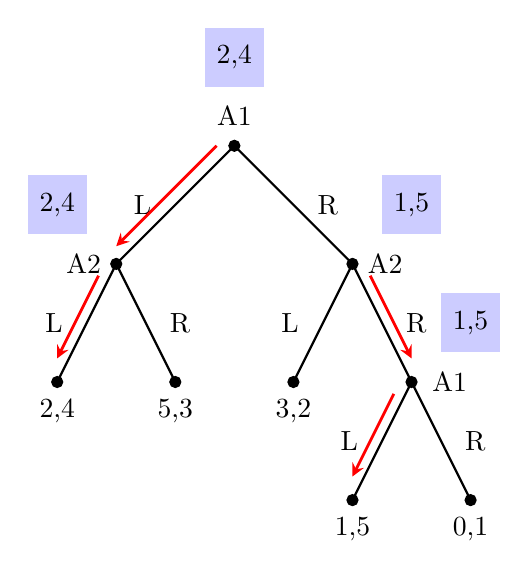
\begin{tikzpicture}[x=0.75cm,y=0.75cm]
     \filldraw[black] (3,6) circle (2pt) node[] at (3, 6.5) {A1};   
     \filldraw[black] (1,4) circle (2pt) node[left=2pt] at (1, 4) {A2};
     \filldraw[black] (5,4) circle (2pt) node[right=2pt] at (5, 4) {A2};   
     \filldraw[black] (0,2) circle (2pt) node[] at (0,1.5) {2,4};
     \filldraw[black] (2,2) circle (2pt) node[] at (2,1.5) {5,3};
     \filldraw[black] (4,2) circle (2pt) node[] at (4,1.5) {3,2};
     \filldraw[black] (6,2) circle (2pt) node[right=4pt] at (6,2) {A1};   
     \filldraw[black] (5,0) circle (2pt) node[] at (5,-0.5) {1,5};
     \filldraw[black] (7,0) circle (2pt) node[] at (7,-0.5) {0,1};
     \draw[black, thick] (3,6) -- (1, 4) node[left=5pt] at (2, 5) {L};
     \draw[black, thick] (3,6) -- (5, 4) node[right=5pt] at (4, 5) {R};   
     \draw[black, thick] (1,4) -- (0, 2) node[left=5pt] at (0.5, 3) {L};
     \draw[black, thick] (1,4) -- (2, 2) node[right=5pt] at (1.5, 3) {R};     
     \draw[black, thick] (5,4) -- (6, 2) node[right=5pt] at (5.5, 3) {R};
     \draw[black, thick] (5,4) -- (4, 2) node[left=5pt] at (4.5, 3) {L};   
     \draw[black, thick] (6,2) -- (5, 0) node[left=5pt] at (5.5, 1) {L};
     \draw[black, thick] (6,2) -- (7, 0) node[right=5pt] at (6.5, 1) {R};
     \visible<2->{\draw [-stealth,red,line width=1pt] (5.7,1.8) -- (5,0.4);}
     \visible<3->{\fill[blue!20!white] (6.5,3.5) rectangle (7.5,2.5) node[black] at (7,3) {1,5};}
     \visible<4->{\draw [-stealth,red,line width=1pt] (5.3,3.8) -- (6,2.4);}
     \visible<5->{\fill[blue!20!white] (5.5,5.5) rectangle (6.5,4.5) node[black] at (6,5) {1,5};}
     \visible<6->{\draw [-stealth,red,line width=1pt] (0.7,3.8) -- (0,2.4);}
     \visible<7->{\fill[blue!20!white] (-0.5,5.5) rectangle (0.5,4.5) node[black] at (0,5) {2,4};}
     \visible<8->{\draw [-stealth,red,line width=1pt] (2.7,6) -- (1,4.3);}
     \visible<9->{\fill[blue!20!white] (2.5,8) rectangle (3.5,7) node[black] at (3,7.5) {2,4};}     
    \end{tikzpicture}
   \end{center}
  \end{frame}


  \begin{frame}{Example: Ultimatum Game}
   \begin{columns}
    \begin{column}{0.6\textwidth}
     \begin{itemize}[<+->]
     \setlength{\itemsep}{1em}
      \item Two agents want to \alert{split $c$ dollars}
      \begin{itemize}[<.->]
       \item A1 offers A2 some amount $x \leq c$
       \item If A2 accepts, outcome is $(c-x,x)$
       \item If A2 rejects, outcome is $(0,0)$
      \end{itemize}
      \item What is A2's best response if $x > 0$?
      \begin{itemize}
       \item Yes
      \end{itemize}
      \item What is A2's best response if $x=0$?
      \begin{itemize}
       \item Indifferent between Yes or No
      \end{itemize}
      \item What are A2's optimal strategies?
      \begin{itemize}
       \item \alert{Option 1}: Yes for all $x \geq 0$
       \item \alert{Option 2}: Yes if $x > 0$, No if $x = 0$
      \end{itemize}
     \end{itemize}
    \end{column}
    \begin{column}{0.4\textwidth}\small
     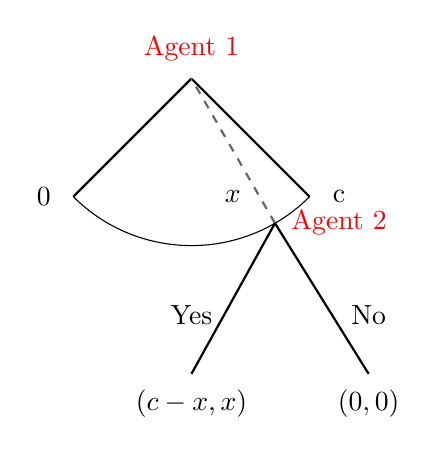
\begin{tikzpicture}[x=0.75cm,y=0.75cm]
      \draw (0,8) arc[start angle=225, end angle=315, radius=2.8284];
      \draw[black, thick] (0,8) -- (2, 10) node[color=red] at (2, 10.5) {Agent 1} node[] at (-0.5,8) {0}; 
      \draw[black, thick] (4,8) -- (2, 10)  node[] at (4.5,8) {c}; 
      \draw[white!40!black, thick, dashed] (3.4142, 7.55051) -- (2, 10); 
      \draw[black, thick] (3.4142, 7.55051) -- (5,5) node[color=red] at (4.5, 7.55051) {Agent 2} node[] at (5, 4.5) {$(0,0)$}  node[] at (5,6) {No}; 
      \draw[black, thick] (3.4142, 7.55051) -- (2,5)  node[] at (2,6) {Yes}  node[] at (2, 4.5) {$(c-x,x)$} node[] at (2.7, 8) {$x$}; 
     \end{tikzpicture}
    \end{column}
   \end{columns}
  \end{frame}

  
  \begin{frame}{SPE of Ultimatum Game}
   \begin{itemize}[<+->]
   \setlength{\itemsep}{1em}
    \item What is A1's optimal strategy for each of A2's optimal strategies?
    \begin{itemize}
    \setlength{\itemsep}{0.5em}
     \item For option 1, A1's optimal strategy is to offer $x = 0$
     \item For option 2, if A1 offers $x=0$, then A1's utility is $0$
     \item If A1 wants to offer any $x > 0$, then A1 must offer 
     $$\underset{x > 0}{\argmax} (c - x)$$
     \item This optimization does not have any optimal solution
     \item \alert{No offer of agent 1 is optimal}
    \end{itemize}
    \item Unique SPE of ultimatum game is \alert{A1 offers 0, and A2 accepts all offers}
   \end{itemize}
  \end{frame}


  \begin{frame}{Example: Discrete Ultimatum Game}
   \begin{itemize}[<+->]
   \setlength{\itemsep}{1.2em}
    \item What are A2's optimal strategies if $c$ is in multiple of cent?
    \begin{itemize}
     \item \alert{Option 1}: Yes for all $x \geq 0$
     \item \alert{Option 2}: Yes if $x > 0$, No if $x = 0$
    \end{itemize}
    \item What are A1's optimal strategies for each of A2's?
    \begin{itemize}
     \item For option 1, offer $x = 0$
     \item For option 2, offer $x = 1$ cent
    \end{itemize}
    \item What are SPE of this modified ultimatum game?
    \begin{itemize}
     \item A1 offers $0$, and A2 accepts all offers
     \item A1 offers $1$ cent, and A2 accepts all offers except $0$
    \end{itemize}
    \item Show that every $\bar{x} \in [0, c]$, there exists NE in which A1 offers $\bar{x}$
    \begin{itemize}
     \item What is agent A2's optimal strategy?
    \end{itemize}
   \end{itemize}
  \end{frame}


  \begin{frame}{Example: Bargaining Game}
   \begin{columns}
    \begin{column}{0.6\textwidth}
     \begin{itemizes}
      \item Two agents want to split $c = 1$ dollar
      \item First, A1 makes her offer
      \item Then, A2 decides to accept or reject
      \item If A2 rejects, then A2 makes new offer
      \item Then, A1 decides to accept or reject 
      \item Let $x = (x_1, x_2)$ denote A1's offer
      \item Let $y = (y_1, y_2)$ denote A2's offer
     \end{itemizes}
    \end{column}
    \begin{column}{0.4\textwidth}\tiny
     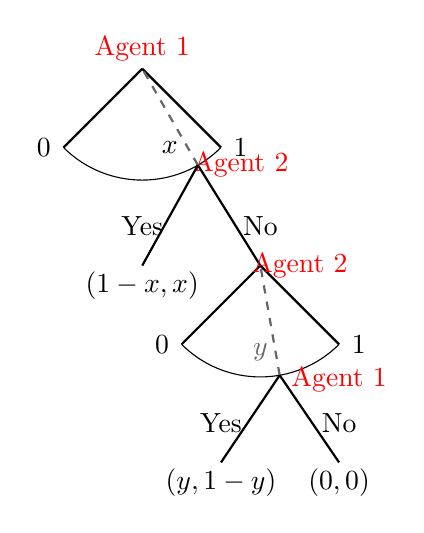
\begin{tikzpicture}[x=0.5cm,y=0.5cm,step=0.5cm]
      \draw (0,8) arc[start angle=225, end angle=315, radius=2.8284];
      \draw[black, thick] (0,8) -- (2, 10) node[color=red] at (2, 10.5) {Agent 1} node[] at (-0.5,8) {0}; 
      \draw[black, thick] (4,8) -- (2, 10)  node[] at (4.5,8) {1};    
      \draw (3,3) arc[start angle=225, end angle=315, radius=2.8284];
      \draw[black, thick] (3,3) -- (5, 5) node[] at (2.5,3) {0}; 
      \draw[black, thick] (7, 3) -- (5, 5) node[] at (7.5,3) {1};    
      \draw[white!40!black, thick, dashed] (3.4142, 7.55051) -- (2, 10); 
      \draw[black, thick] (3.4142, 7.55051) -- (5,5) node[color=red] at (4.5, 7.55051) {Agent 2} node[color=red] at (6, 5) {Agent 2}  node[] at (5,6) {No}; 
      \draw[black, thick] (3.4142, 7.55051) -- (2,5)  node[] at (2,6) {Yes}  node[] at (2, 4.5) {$(1-x, x)$} node[] at (2.7, 8) {$x$}; 
      \draw[white!40!black, thick, dashed] (5.4911512, 2.214543039) -- (5,5) node[color=red] at (7, 2.1) {Agent 1}  node[] at (5, 2.8) {$y$}; 
      \draw[black, thick] (5.4911512, 2.214543039) -- (7,0) node[] at (7,1) {No} node[] at (7, -0.5) {$(0,0)$}; 
      \draw[black, thick] (5.4911512, 2.214543039) -- (4,0) node[] at (4,1) {Yes} node[] at (4, -0.5) {$(y, 1-y)$};      
     \end{tikzpicture}
    \end{column}
   \end{columns}
  \end{frame}


  \begin{frame}{Backward Induction for Bargaining Game}
   \begin{itemize}[<+->]
   \setlength{\itemsep}{0.5em}
    \item Second round is ultimatum game with \alert{unique SPE}
    \begin{itemize}
     \item A2 offers $0$, and A1 accepts all offers 
    \end{itemize}
    \item What is A2's optimal strategy in round 1's subgame?
    \begin{itemize}
     \item \alert{Option 1}: If $x_2 \leq 1$, reject 
     \item \alert{Option 2}: If $x_2=1$, accept, and reject otherwise
    \end{itemize}
    \item What are A1's optimal strategies in round 1 for each of A2's?
    \begin{itemize}
     \item For both options, A1 is indifferent between all strategies
    \end{itemize}
    \item How many SPE does this game have?
    \begin{itemize}
     \item Infinitely many! In all SPE, A2 gets everything (\alert{Last mover's advantage})
     \item In every SPE, agent who makes offer in last round gets everything
    \end{itemize}
   \end{itemize}
  \end{frame}


  \begin{frame}{Example: Discounted Bargaining Game}
   \begin{columns}
    \begin{column}{0.6\textwidth}
     \begin{itemize}[<+->]
     \setlength{\itemsep}{1em}
      \item Utilities are discounted by $0 < \delta_i < 1$
      \item What is unique SPE of (1)?
      \begin{itemize}
       \item A2 offers $y_1=0$ and A1 accepts all offers
      \end{itemize}
      \item What are optimal strategies in (2)?
      \begin{itemize}
       \item \alert{Option 1}: Yes if $x_2 \geq \delta_2$, No otherwise
       \item \alert{Option 2}: Yes if $x_2 > \delta_2$, No otherwise
      \end{itemize}
      \item What are optimal strategies in (3)?
      \begin{itemize}
       \item For option 1, offer $x_2=\delta_2$
       \item For option 2, there is no optimal strategy
      \end{itemize}
     \end{itemize}
    \end{column}
    \begin{column}{0.4\textwidth}\tiny
     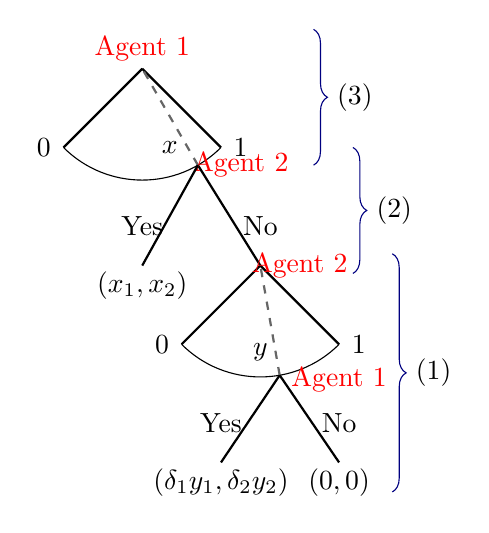
\begin{tikzpicture}[x=0.5cm,y=0.5cm,step=0.5cm]
      \draw (0,8) arc[start angle=225, end angle=315, radius=2.8284];
      \draw[black, thick] (0,8) -- (2, 10) node[color=red] at (2, 10.5) {Agent 1} node[] at (-0.5,8) {0}; 
      \draw[black, thick] (4,8) -- (2, 10)  node[] at (4.5,8) {1}; 
      \draw (3,3) arc[start angle=225, end angle=315, radius=2.8284];
      \draw[black, thick] (3,3) -- (5, 5) node[] at (2.5,3) {0}; 
      \draw[black, thick] (7, 3) -- (5, 5) node[] at (7.5,3) {1}; 
      \draw[white!40!black, thick, dashed] (3.4142, 7.55051) -- (2, 10); 
      \draw[black, thick] (3.4142, 7.55051) -- (5,5) node[color=red] at (4.5, 7.55051) {Agent 2} node[color=red] at (6, 5) {Agent 2}  node[] at (5,6) {No}; 
      \draw[black, thick] (3.4142, 7.55051) -- (2,5)  node[] at (2,6) {Yes}  node[] at (2, 4.5) {$(x_1, x_2)$} node[black] at (2.7, 8) {$x$}; 
      \draw[white!40!black, thick, dashed] (5.4911512, 2.214543039) -- (5,5) node[color=red] at (7, 2.1) {Agent 1}  node[black] at (5, 2.8) {$y$}; 
      \draw[black, thick] (5.4911512, 2.214543039) -- (7,0) node[] at (7,1) {No} node[] at (7, -0.5) {$(0,0)$}; 
      \draw[black, thick] (5.4911512, 2.214543039) -- (4,0) node[] at (4,1) {Yes} node[] at (4, -0.5) {$(\delta_1 y_1, \delta_2 y_2)$};    
      \draw [blue!50!black,decorate, decoration = {brace,raise=5pt, amplitude=5pt}] (6,11) --  (6,7.55051) node[pos=0.5,right=10pt,black]{$(3)$};
      \draw [blue!50!black,decorate, decoration = {brace,raise=5pt, amplitude=5pt}] (7,8) --  (7,4.8) node[pos=0.5,right=10pt,black]{$(2)$};
      \draw [blue!50!black,decorate, decoration = {brace,raise=5pt, amplitude=5pt}] (8,5.3) --  (8,-0.75) node[pos=0.5,right=10pt,black]{$(1)$};
     \end{tikzpicture}
    \end{column}
   \end{columns}
  \end{frame}


  \begin{frame}{Unique SPE of Discounted Bargaining Game}
   \begin{itemize}
   \setlength{\itemsep}{1.3em}
    \item What are SPE \alert{strategies}?
    \begin{itemize}
     \item Agent 1's proposes $(1-\delta_2, \delta_2)$
     \item Agent 2 only accepts proposals with $x_2 \geq \delta_2$
     \item Agent 2 proposes $(0, 1)$ after any history in which1's proposal is rejected
     \item Agent 1 accepts all proposals of Agent 2
    \end{itemize}
    \item What is SPE \alert{outcome} of game?
    \begin{itemize}
     \item Agent 1 proposes $(1-\delta_2, \delta_2)$
     \item Agent 2 accepts
     \item Resulting utilities are $(1-\delta_2, \delta_2)$
    \end{itemize}
    \item Desirability of earlier agreement yields positive utility for agent 1
   \end{itemize}
  \end{frame}


  \begin{frame}{Limitation of Backward Induction}
   \begin{itemize}
    \item If there are ties, how they are broken affects what happens up in tree
   \end{itemize}
   \begin{center}\tiny
    \begin{tikzpicture}[x=0.75cm,y=0.75cm,step=0.75cm]
     \filldraw[black] (3,4) circle (2pt) node[color=red] at (3,4.5){A1};
     \filldraw[black] (1,2) circle (2pt) node[color=red] at (0, 2){A2};
     \filldraw[black] (5,2) circle (2pt) node[color=red] at (6, 2){A2};
     \filldraw[black] (0,0) circle (2pt) node[] at (0, -0.5) {3,2};
     \filldraw[black] (2,0) circle (2pt) node[] at (2, -0.5) {2,3};
     \filldraw[black] (4,0) circle (2pt) node[] at (4, -0.5) {4,1};
     \filldraw[black] (6,0) circle (2pt) node[] at (6, -0.5) {0,1};
     \draw[black, thick] (3,4) -- (1, 2);
     \draw[black, thick] (3,4) -- (5, 2); 
     \draw[black, thick] (1,2) -- (0, 0); 
     \draw[black, thick] (1,2) -- (2, 0);
     \draw[black, thick] (5,2) -- (4, 0); 
     \draw[black, thick] (5,2) -- (6, 0);
     \visible<3->{\draw [-stealth,cyan, line width = 1pt](2.5,3.8) -- (1.2,2.5);
     \draw [-stealth,cyan, line width = 1pt](1.5,1.8) -- (2.3,0.2);
     \draw [-stealth,cyan, line width = 1pt](5.3,1.8) -- (6.1,0.2);}
     \visible<2->{\draw [-stealth,black, line width = 1pt](3.5,3.8) -- (4.8,2.5);
     \draw [-stealth,black, line width = 1pt](1.3,1.8) -- (2.1,0.2);
     \draw [-stealth,black, line width = 1pt](4.7,1.8) -- (3.9,0.2);}
     \visible<4->{\draw [-stealth,darkgreen, line width = 1pt](1.7,1.8) -- (2.5,0.2);
     \draw [-stealth,darkgreen, line width = 1pt](2.2,3.8) -- (0.9,2.5) node[darkgreen, anchor=east] at (1,3) {$0.12345$};
     \draw [-stealth,darkgreen, line width = 1pt](3.8,3.8) -- (5.1,2.5) node[darkgreen, anchor=west] at (5,3) {$0.87655$};
     \draw [-stealth,darkgreen, line width = 1pt](4.5,1.8) -- (3.7,0.2) node[darkgreen] at (3.5,1) {$0.5$};
     \draw [-stealth,darkgreen, line width = 1pt](5.5,1.8) -- (6.3,0.2) node[darkgreen] at (6.5,1) {$0.5$};}
    \end{tikzpicture}
   \end{center}
  \end{frame}

 \section{Imperfect-info Extensive-form Games}
 
  \begin{frame}{Imperfect-info Games: Motivation}
   \begin{itemize}[<+->]
   \setlength{\itemsep}{1.2em}
    \item So far, we have allowed agents to specify action they take at every choice node
    \item This implies that agents know the node they are in and all prior choices
    \item This is why we call these games \alert{perfect-information} games
    \item However, this might not be the case in all environments
   \end{itemize}
  \end{frame}
  
    \begin{frame}{Imperfect-info Games: Motivation (cont.)}
   \begin{itemize}[<+->]
   \setlength{\itemsep}{1.2em}
    \item We may want to model agents with \alert{partial or no knowledge} of others' actions
    \item We may even want to model agents with \alert{limited memory} of their \alert{own} past actions
    \item \alert{Imperfect-info} games in extensive form address this limitation
    \item In such games, each agent's choice nodes are partitioned into \alert{information sets}
    \item If two nodes are in same info set, then agent cannot distinguish between them
   \end{itemize}
  \end{frame}
 
  \begin{frame}{Imperfect-info Extensive-form Games: Definition}
   \begin{itemize}
   \setlength{\itemsep}{1.5em}
    \item $N$, $A$, $H$, $Z$, $\alpha$, $\beta$, $\rho$, $u$ are the same as before
    \item $I = (I_1,...,I_n)$, where $I_i = (I_{i,1},...,I_{i,k_i})$ is a partition of $\{h \in H : \alpha(h) = i\}$
    \item If $h, h^\prime$ are in the same \alert{equivalence class} $I_{i,j}$, then $\beta(h) = \beta(h^\prime)$
    \item Perfect-info games are imperfect-info games with singleton equivalence classes
   \end{itemize}
  \end{frame}


  \begin{frame}{Example: Prisoners' Dilemma in Extensive Form}
   \begin{columns}
    \begin{column}{0.45\textwidth}
     \begin{itemizes}
      \item P1 decides on D or C
      \item P2 then decides on D or C\\(without observing P1's decision)
     \end{itemizes}
    \end{column}
    \begin{column}{0.55\textwidth}   
     \begin{center}\small
      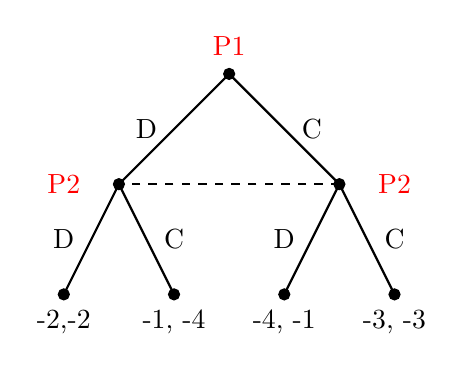
\begin{tikzpicture}[x=0.7cm,y=0.7cm,step=0.7cm]
       \filldraw[black] (3,4) circle (2pt) node[color=red] at (3,4.5){P1};
       \filldraw[black] (1,2) circle (2pt) node[color=red] at (0, 2){P2};
       \filldraw[black] (5,2) circle (2pt) node[color=red] at (6, 2){P2};
       \filldraw[black] (0,0) circle (2pt) node[] at (0, -0.5) {-2,-2};
       \filldraw[black] (2,0) circle (2pt) node[] at (2, -0.5) {-1, -4};
       \filldraw[black] (4,0) circle (2pt) node[] at (4, -0.5) {-4, -1};
       \filldraw[black] (6,0) circle (2pt) node[] at (6, -0.5) {-3, -3};
       \draw[black, thick] (3,4) -- (1, 2) node[] at (1.5, 3) {D}; 
       \draw[black, thick] (3,4) -- (5, 2) node[] at (4.5, 3) {C}; 
       \draw[black, thick] (1,2) -- (0, 0) node[] at (0, 1) {D}; 
       \draw[black, thick] (1,2) -- (2, 0) node[] at (2, 1) {C}; 
       \draw[black, thick] (5,2) -- (4, 0) node[] at (4, 1) {D}; 
       \draw[black, thick] (5,2) -- (6, 0) node[] at (6, 1) {C};
       \draw[black, thick, dashed] (5,2) -- (1, 2);   
      \end{tikzpicture}
     \end{center}
    \end{column}
   \end{columns}
  \end{frame}
  
  
 \section{Randomized Strategies in Extensive-form Games}
 
  \begin{frame}{Pure, Mixed, and Behavioral Strategies}
   \begin{itemize}[<+->]
   \setlength{\itemsep}{1em}
    \item \alert{Pure strategies} of agent $i$ consists of $\prod_{I_{i,j} \in I_i} \beta(I_{i,j})$
    \item \alert{Mixed strategies} define randomization over pure strategies
    \item \alert{Behavioral strategy} define independent randomization at each info set
    \item Mixed strategy is \alert{distribution over vectors} (each vector describing a pure strategy)
    \item Behavioral strategy is a \alert{vector of distributions}
    \item In general, expressive power of behavioral and mixed strategies are noncomparable
    \begin{itemize}
     \item In some games, there are outcomes that are achieved via mixed but not any behavioral strategies
     \item And in some games it is the other way around
    \end{itemize}
   \end{itemize}
  \end{frame}
  
   
  \begin{frame}{Mixed vs Behavioral Strategies: Example I}
   \begin{columns}
    \begin{column}{0.6\textwidth}
     \begin{itemize}[<+->]
     \setlength{\itemsep}{1.2em}
      \item Give behavioral strategy for A1
      \begin{itemize}
       \item L w.p. 0.2 and L w.p. 0.5
      \end{itemize}
      \item Give mixed strategy for A1 that is not behavioral strategy
      \begin{itemize}
       \item (L, L) w.p. 0.4 and (R, R) w.p. 0.6
       \item Why this is not behavioral strategy?
      \end{itemize}
      \item In this game, every behavioral strategy \alert{corresponds to} a mixed strategy and vice versa (more on this soon)
     \end{itemize}
    \end{column}
    \begin{column}{0.4\textwidth}   
     \begin{center}\scriptsize
      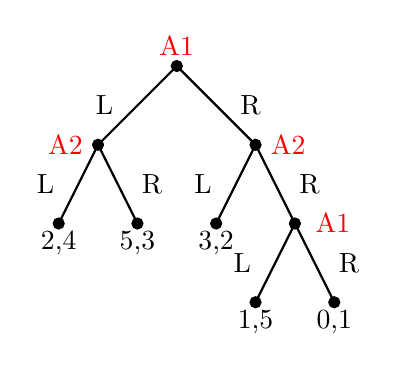
\begin{tikzpicture}[x=0.5cm,y=0.5cm,step=0.5cm]
       \filldraw[black] (3,6) circle (2pt) node[red] at (3, 6.5) {A1};   
       \filldraw[black] (1,4) circle (2pt) node[red, left=2pt] at (1, 4) {A2};
       \filldraw[black] (5,4) circle (2pt) node[red, right=2pt] at (5, 4) {A2};   
       \filldraw[black] (0,2) circle (2pt) node[] at (0,1.5) {2,4};
       \filldraw[black] (2,2) circle (2pt) node[] at (2,1.5) {5,3};
       \filldraw[black] (4,2) circle (2pt) node[] at (4,1.5) {3,2};
       \filldraw[black] (6,2) circle (2pt) node[red, right=4pt] at (6,2) {A1};   
       \filldraw[black] (5,0) circle (2pt) node[] at (5,-0.5) {1,5};
       \filldraw[black] (7,0) circle (2pt) node[] at (7,-0.5) {0,1};
       \draw[black, thick] (3,6) -- (1, 4) node[left=5pt] at (2, 5) {L};
       \draw[black, thick] (3,6) -- (5, 4) node[right=5pt] at (4, 5) {R};   
       \draw[black, thick] (1,4) -- (0, 2) node[left=5pt] at (0.5, 3) {L};
       \draw[black, thick] (1,4) -- (2, 2) node[right=5pt] at (1.5, 3) {R};     
       \draw[black, thick] (5,4) -- (6, 2) node[right=5pt] at (5.5, 3) {R};
       \draw[black, thick] (5,4) -- (4, 2) node[left=5pt] at (4.5, 3) {L};   
       \draw[black, thick] (6,2) -- (5, 0) node[left=5pt] at (5.5, 1) {L};
       \draw[black, thick] (6,2) -- (7, 0) node[right=5pt] at (6.5, 1) {R};    
      \end{tikzpicture}
     \end{center}
    \end{column}
   \end{columns}
  \end{frame}
  
  \begin{frame}{Mixed vs Behavioral Strategies: Example II}
   \begin{columns}
    \begin{column}{0.6\textwidth}
     \begin{itemize}[<+->]
     \setlength{\itemsep}{1.2em}
      \item What is mixed-strategy NE of this game?
      \begin{itemize}
       \item (R, D) with outcome utilities (2,2)
      \end{itemize}
      \item What is A1's expected utility for $(p, 1-p)$?
      \begin{itemize}
       \item $p^2 + 100p(1-p) + 2(1-p)$
      \end{itemize}
      \item What is A1's best response? 
      \begin{itemize}
       \item $p$ $=$ 98/198
      \end{itemize}       
      \item  What is behavioral NE of this game?
      \begin{itemize}
       \item ((98/198, 100/198), (0, 1))
      \end{itemize}
     \end{itemize}
    \end{column}
    \begin{column}{0.4\textwidth}   
     \begin{center}\scriptsize
      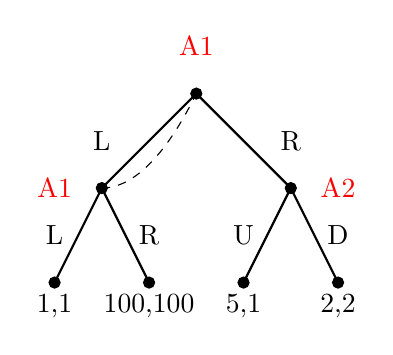
\begin{tikzpicture}[x=0.6cm,y=0.6cm]
       \filldraw[black] (3,4) circle (2pt) node[color=red] at (3, 5) {A1};
       \filldraw[black] (1,2) circle (2pt) node[color=red] at (0, 2) {A1};
       \filldraw[black] (5,2) circle (2pt) node[color=red] at (6, 2) {A2}; 
       \filldraw[black] (0,0) circle (2pt) node[] at (0, -0.5) {1,1};
       \filldraw[black] (2,0) circle (2pt) node[] at (2, -0.5) {100,100};
       \filldraw[black] (4,0) circle (2pt) node[] at (4, -0.5) {5,1};
       \filldraw[black] (6,0) circle (2pt) node[] at (6, -0.5) {2,2};
       \draw[black, thick] (3,4) -- (1, 2) node[] at (1, 3) {L}; 
       \draw[black, thick] (3,4) -- (5, 2) node[] at (5, 3) {R}; 
       \draw[black, thick] (5,2) -- (6,0) node[] at (6, 1) {D}; 
       \draw[black, thick] (5,2) -- (4,0) node[] at (4, 1) {U}; 
       \draw[black, thick] (1,2) -- (0, 0) node[] at (0, 1) {L}; 
       \draw[black, thick] (1,2) -- (2, 0) node[] at (2, 1) {R}; 
       \draw[dashed] (1,2) parabola (3,4);
      \end{tikzpicture}
     \end{center}
    \end{column}
   \end{columns}  
  \end{frame}  
  
  \begin{frame}{Perfect Recall}
   \begin{itemize}[<+->]
   \setlength{\itemsep}{1.2em}
    \item Strategies that induce same distribution on outcomes, for fixed strategy profile of others, are called \alert{equivalent} strategies
    \item If all agents remember all their own actions, game is a game of \alert{perfect recall}
    \item In such games, any mixed strategy of given agent can be replaced by an \alert{equivalent} behavioral strategy
    \item And any behavioral strategy can be replaced by an \alert{equivalent} mixed strategy
   \end{itemize}
  \end{frame}
  
  
  \begin{frame}{Subgame Perfection and Imperfect Information}
   \begin{center}\tiny
    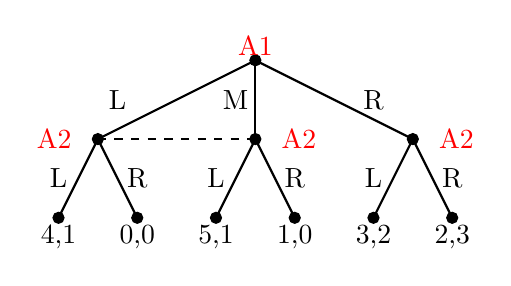
\begin{tikzpicture}[x=0.5cm,y=0.5cm,step=0.5cm]
     \filldraw[black] (5,4) circle (2pt) node[anchor=north, yshift=12pt, color=red]{A1};
     \filldraw[black] (1,2) circle (2pt) node[anchor=east, xshift=-6pt, color=red]{A2};
     \filldraw[black] (5,2) circle (2pt) node[anchor=west, xshift=6pt, color=red]{A2};
     \filldraw[black] (9,2) circle (2pt) node[anchor=west, xshift=6pt, color=red]{A2};
     \filldraw[black] (0,0) circle (2pt) node[] at (0,-0.5) {4,1}; 
     \filldraw[black] (2,0) circle (2pt) node[] at (2,-0.5) {0,0};
     \filldraw[black] (4,0) circle (2pt) node[] at (4,-0.5) {5,1};
     \filldraw[black] (6,0) circle (2pt) node[] at (6,-0.5) {1,0};
     \filldraw[black] (8,0) circle (2pt) node[] at (8,-0.5) {3,2};
     \filldraw[black] (10,0) circle (2pt) node[] at (10,-0.5) {2,3};
     \draw[black, thick] (5,4) -- (1, 2) node[] at (1.5, 3) {L};
     \draw[black, thick] (5,4) -- (5, 2) node[] at (4.5, 3) {M};
     \draw[black, thick] (5,4) -- (9, 2) node[] at (8, 3) {R};
     \draw[black, thick, dashed] (1,2) -- (5, 2); 
     \draw[black, thick] (1,2) -- (0, 0) node[] at (0, 1) {L}; 
     \draw[black, thick] (1,2) -- (2, 0) node[] at (2, 1) {R};
     \draw[black, thick] (5,2) -- (4, 0) node[] at (4, 1) {L};
     \draw[black, thick] (5,2) -- (6, 0) node[] at (6, 1) {R};
     \draw[black, thick] (9,2) -- (8, 0) node[] at (8, 1) {L};
     \draw[black, thick] (9,2) -- (10, 0) node[] at (10, 1) {R};    
    \end{tikzpicture}
   \end{center}
   \begin{itemize}[<+->]
    \item There are two subgames: game itself and subgame after agent 1 plays R
    \begin{itemize}
     \item (R, (R,R)) is NE and SPE
    \end{itemize}
    \item But, why should 2 play R after 1 plays L or M?
    \begin{itemize}
     \item This is \alert{non-credible threat} 
    \end{itemize}
    \item There are more sophisticated equilibrium refinements that rule this out
    \begin{itemize}
     \item They explicitly model agents' beliefs on where they are for every info set     
     \item E.g., sequential equilibrium, perfect Bayesian equilibrium
    \end{itemize}
   \end{itemize}
  \end{frame}
   
  
  \begin{frame}{Acknowledgment}
   \begin{itemize}
   \setlength{\itemsep}{1em}
    \item This lecture is a slightly modified version of ones prepared by
    \begin{itemize}
     \item Asu Ozdaglar \href{https://ocw.mit.edu/courses/electrical-engineering-and-computer-science/6-254-game-theory-with-engineering-applications-spring-2010/index.htm}{[MIT 6.254]}
     \item Vincent Conitzer \href{https://courses.cs.duke.edu/spring16/compsci590.4/}{[Duke CPS 590.4]}
    \end{itemize}
    \item Hadi Omidi helped with importing slides from PowerPoint to \LaTeX
   \end{itemize}
  \end{frame}

\end{document}
